%%%%%%%%%%%%%%%%%%%%%%% file template.tex %%%%%%%%%%%%%%%%%%%%%%%%%
%
% This is a general template file for the LaTeX package SVJour3
% for Springer journals.          Springer Heidelberg 2010/09/16
%
% Copy it to a new file with a new name and usFe it as the basis
% for your article. Delete % signs as needed.
%
% This template includes a few options for different layouts and
% content for various journals. Please consult a previous issue of
% your journal as needed.
%
%%%%%%%%%%%%%%%%%%%%%%%%%%%%%%%%%%%%%%%%%%%%%%%%%%%%%%%%%%%%%%%%%%%
%
% First comes an example EPS file -- just ignore it and
% proceed on the \documentclass line
% your LaTeX will extract the file if required

\RequirePackage{fix-cm}
%
%\documentclass{svjour3}                     % onecolumn (standard format)
%\documentclass[smallcondensed]{svjour3}     % onecolumn (ditto)
%\documentclass[smallextended]{svjour3}       % onecolumn (second format)
\documentclass[twocolumn]{svjour3}          % twocolumn
%
\smartqed  % flush right qed marks, e.g. at end of proof
%
\usepackage{graphicx}
\usepackage{amsmath} 
\usepackage{amssymb}
\usepackage{tensor} 
\usepackage{cite}
\usepackage{floatrow}
\usepackage{blindtext}
%
% \usepackage{mathptmx}      % use Times fonts if available on your TeX system
%
% insert here the call for the packages your document requires
%\usepackage{latexsym}
% etc.
%
% please place your own definitions here and don't use \def but
% \newcommand{}{}
%
% Insert the name of "your journal" with
% \journalname{myjournal}
%
\newcommand{\Vol}{\mathop{\rm Vol}}
\newcommand{\diff}{\textit{diff}}
\newcommand{\affine}{\mathop{\it affine}}
\newcommand{\manifold}{\mathop{\it manifold}}
\newcommand{\Ueps}{U_{\epsilon}}
\newcommand{\limeps}{\lim_{\epsilon \to 0}}
\newcommand{\delx}{\Delta x}
\newcommand{\R}{\mathbb{R}}
\newcommand{\Rtwo}{{\mathbb{R}}^2}
\newcommand{\Rn}{{\mathbb{R}}^n}
\newcommand{\Rm}{{\mathbb{R}}^m}
\newcommand{\Proj}{\mathrm{P}{\,}}
\newcommand{\Ima}{\mathrm{Im}{\,}}
\newcommand{\ProjNonOrth}[2]{\tensor*{\Proj}{^{#1}_{#2}}}
\newcommand{\Laplace}{\mathrm{\Delta}}
\newcommand{\LaplaceBeltrami}{\mathrm{\Delta_{{LB}}}}
%\newcommand{\partderiv}[2]{\frac{\partial #1}{\partial #2}}
\newcommand{\partderiv}[2]{\partial_{#2} {#1}}
\newcommand{\extr}[1]{\mathrm{extr}_{#1}}
\newcommand{\toreal}{\rightarrow\R}
\newcommand{\toeuclidean}[1]{\rightarrow\R^{#1}}
\newcommand{\CovariantDiffManif}[1]{\nabla^{#1}}
\newcommand{\CovariantDerivManif}[2]{\tensor*{\nabla}{^{#1}_{#2}}}
\newcommand{\CovariantDiff}{\nabla}
\newcommand{\CovariantDeriv}[1]{\nabla_{#1}}
\newcommand{\Diff}{\mathrm{d}}
\newcommand{\TangentSpaceArg}[2]{{T_{#2}}{#1}}
\newcommand{\CotangentSpaceArg}[2]{\tensor*{T}{^{*}_{#2}}{#1}}
\newcommand{\TangentBundle}[1]{T{#1}}
\newcommand{\CotangentBundle}[1]{\tensor*{T}{^{*}}{#1}}
\newcommand{\FRScalar}{BR_{\mathrm{scalar}}}
\newcommand{\FRMean}{BR_{\mathrm{mean}}}
\newcommand {\tr}{{\,}\mathrm{tr}{\,}}
\newcommand {\Preimage}[2]{{#2}^*{#1}}
\newcommand \TArgPreimage[3]{\Preimage{\TangentSpaceArg{#1}{#2}}{#3}}
\newcommand {\DiffSpaceArg}[4]{\CotangentSpaceArg{#1}{#2}\otimes \TArgPreimage{#2}{#3}}
\newcommand {\HessianSpaceP}[3]{\CotangentSpaceP{#1}\otimes \CotangentSpaceP{#1}\otimes \TpPreimage{#2}{#3}}

\newcommand \TPreimage[2]{\Preimage{\TangentBundle{#1}}{#2}}
\newcommand \CotPreimage[2]{\Preimage{\CotangentBundle{#1}}{#2}}
\newcommand \CotPPreimage[2]{\Preimage{\CotangentSpaceP{#1}}{#2}}
\newcommand {\DiffSpace}[3]{\CotangentBundle{#1}\otimes \TPreimage{#2}{#3}}
\newcommand {\HessianSpace}[2]{\CotangentBundle{#1}\otimes \CotangentBundle{#1}\otimes \TangentBundle{#2}}
\newcommand {\HessianSpaceF}[3]{\CotangentBundle{#1}\otimes \CotangentBundle{#1}\otimes \TPreimage{#2}{#3}}
\newcommand {\HessianSpaceFArg}[3]{\CotangentBundle{#1}\otimes \CotangentBundle{#1}\otimes \TPreimage{#2}{#3}}

\newcommand {\bigeps}{\mathcal{E}}

\begin{document}

	
\title{Manifold blob detection by interpretation of blob detection as non-linearity seeking
}

%\titlerunning{Short form of title}        % if too long for running head

\author{Aleksei Shestov         \and
        Mikhail Kumskov %etc.
}

%\authorrunning{Short form of author list} % if too long for running head

\institute{A. Shestov \at
              Lomonosov Moscow State University, Faculty of Mechanics and Mathematics, Russia, 119991, Moscow, GSP-1, 1 Leninskiye Gory, Main Building \\
              \email{shestov.msu@gmail.com}           %  \\
%             \emph{Present address:} of F. Author  %  if needed
           \and
           M. Kumskov \at
              Lomonosov Moscow State University, Faculty of Mechanics and Mathematics, Russia, 119991, Moscow, GSP-1, 1 Leninskiye Gory, Main Building \\
              \email{mkumskov@gmail.com}
}

\date{Received: date / Accepted: date}
% The correct dates will be entered by the editor
\twocolumn[\begin{@twocolumnfalse}
\maketitle

\begin{abstract}
This paper is devoted to the problem of blob detection generalization for manifold-valued images. Our solution is based on a new interpretation of blob detection, which is in agreement with intuitive understanding of the algorithm. We interpret blob response functions as a measure of local non-linearity. This interpretation with minor modifications is extended to the manifold case, what allows us to define the algorithm for this case. Then we derive an expression of the manifold blob response functions through the image Hessian. This gives the manifold algorithm a form similar to the grayscale case. Finally, we provide experiments for the case of vector-valued images on 2D surfaces: the algorithm is tested for physico-chemical properties of chemical compounds.
\keywords{Blob Detection \and Image Processing \and Manifold-valued Images \and Vector-valued Images \and Differential Geometry}
% \PACS{PACS code1 \and PACS code2 \and more}
% \subclass{MSC code1 \and MSC code2 \and more}
\end{abstract}
\end{@twocolumnfalse}]
\section{Introduction}
\label{intro}
%
Non-Euclidean data appears in many applications and practical cases. In chemical compounds classification, 3d reconstruction, 3d models recognition, action recognition, medical images processing we deal with vector-valued or manifold-valued functions defined on manifolds. Circle-valued images (periodic data) are processed in interferometric synthetic aperture radar \cite{CircleData1, CircleData2}, in applications involving the phase of Fourier transformed data \cite{CircleData3} or the hue-component of an image. Spherical are met when dealing with 3D directional information \cite{SphereData1, SphereData2} or with color images in the chromaticity-brightness (CB) color space \cite{SphereData3} (see Fig. \ref{fig:example1}). SO(3)-valued data are processed in electron backscattered tomography \cite{SO3Data1, SO3Data2}. Images with symmetric positive definite matrices as values appear in DT-MRI imaging \cite{SPDMatrixData1, SPDMatrixData2} or in processing covariance matrices associated to image pixels \cite{SPDMatrixData3}. One approach to the manifold data processing development is a generalization of grayscale image processing methods. 

\begin{figure}[!ht]
\setlength{\lineskip}{0pt}
\vspace{-4.0cm}
  \centering
   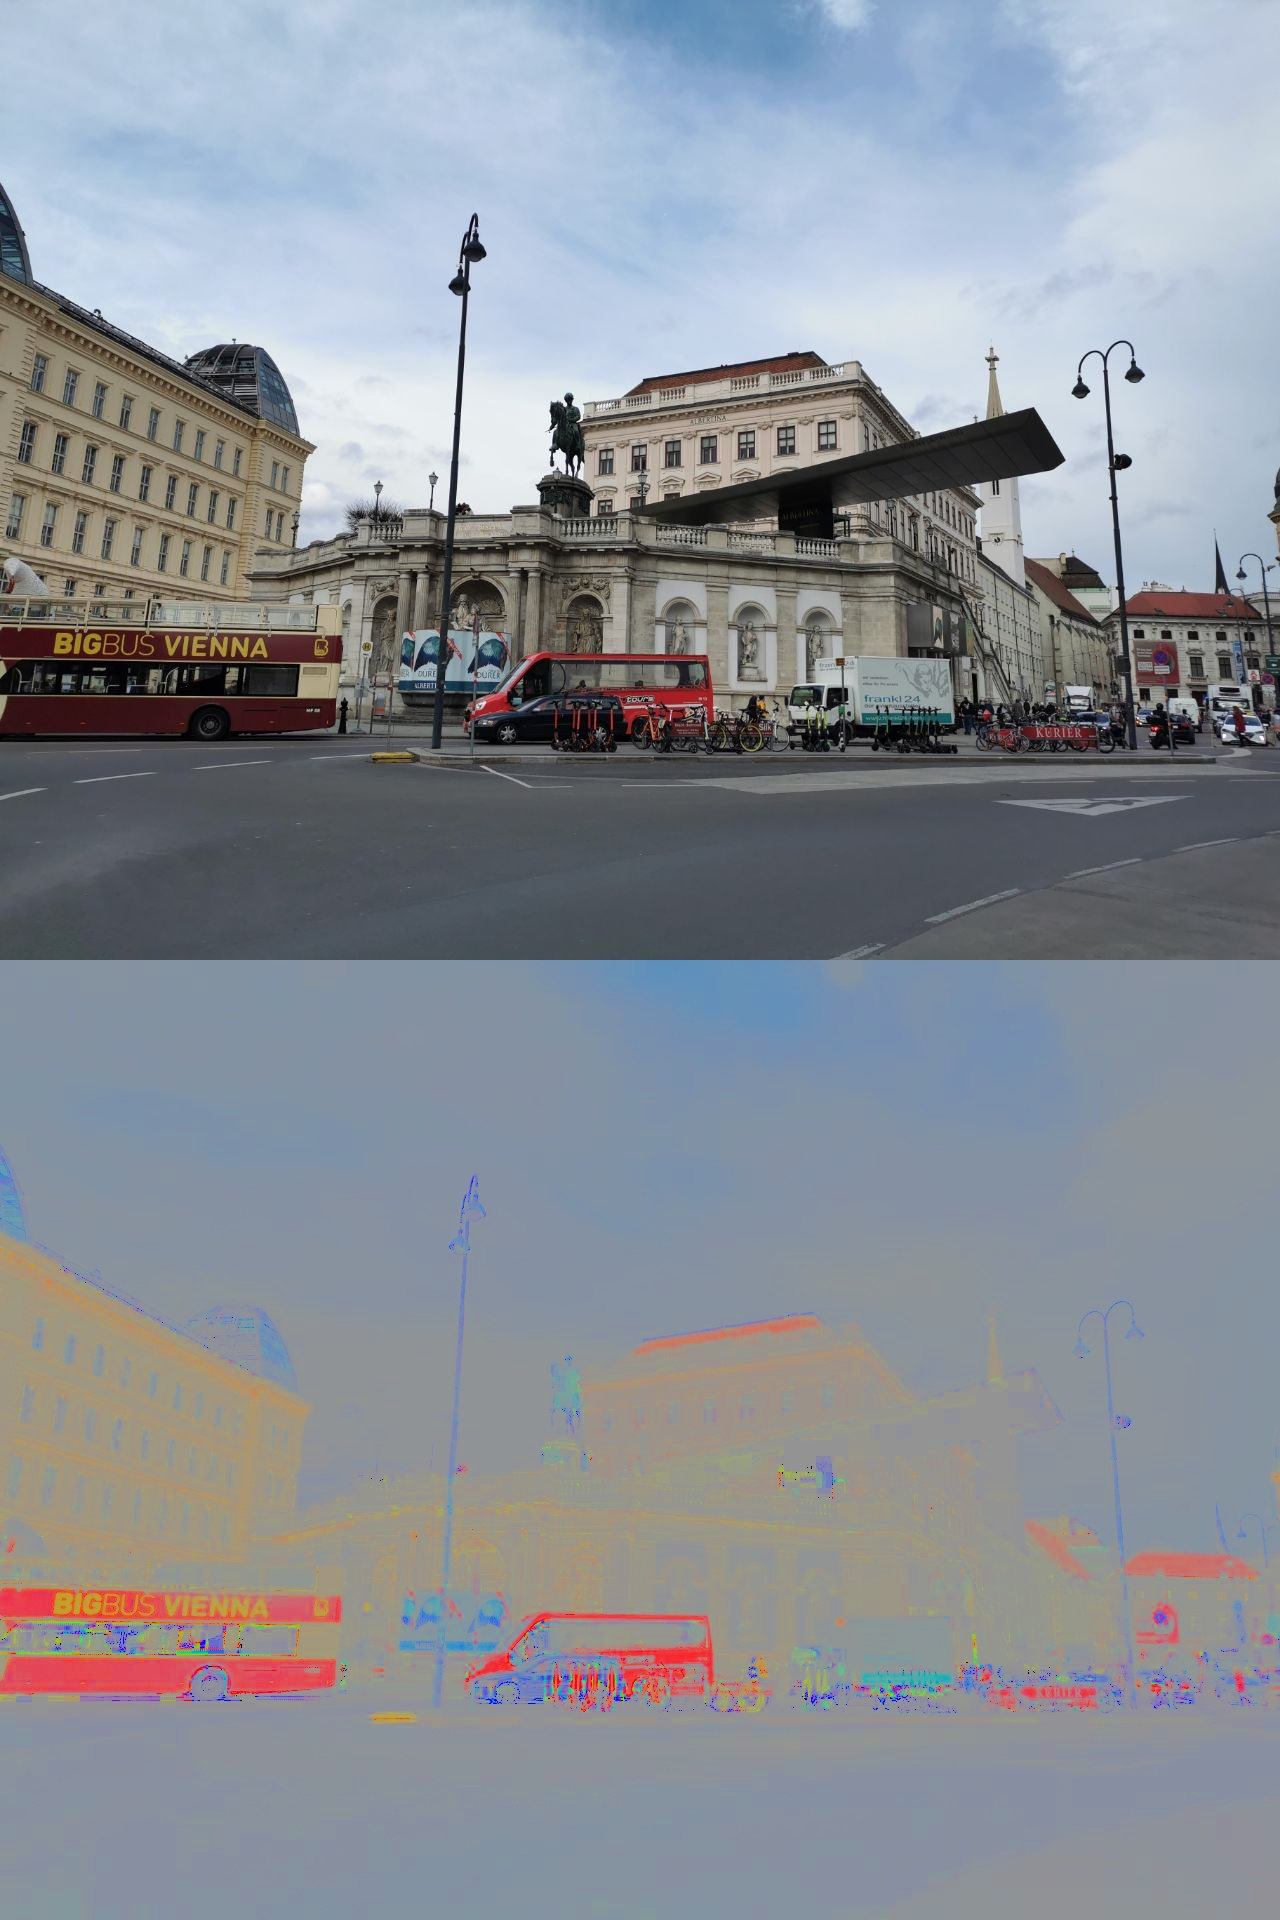
\includegraphics[scale=0.25,natwidth=1280,natheight=1920]{8.jpg} 
  \caption{An image in the RGB space and its chromaticity component under it.}
  \label{fig:example1}
 \end{figure} 

Blob detection \cite{blob} is a widely used method of keypoints detection in grayscale images. It has applications in 3D face recognition, object recognition, panorama stitching, 3D scene modeling, tracking, action recognition, medical images processing \cite{GenLapl, GenLaplNucl, VesselEnh, CHEF}, etc. The algorithm consists of 3 steps: first, a scale-space is constructed from the original image, second, a blob response is calculated from the scale-space, third, blobs centers are sought as local extremums of the blob response in the spatial and scale dimensions. A heuristic understanding is that blob detection aims to find regions which are different from surroundings and with similar intensity inside, i.e. blobs. For a generalization of the algorithm to non-scalar-valued images the main question is generalizing the blob response functions. The reason of it is that they are calculated from the image Hessian, and the image Hessian is not a matrix in the non-scalar-valued case.
\\
Our goal is to develop a generalization of blob detection for the general setting of an image being a map between Riemannian manifolds $I(x):X \to Y$. Note that this general setting contains also a more frequent case of $Y = \Rn $. We need to pick key algorithm properties which we want to preserve in the generalization. In order to do this we propose a new interpretations of the blob response functions, which are in agreement with heuristic algorithm understanding and which can be extended to the manifold case. In our interpretation the blob response functions show how different is the image from being a linear function at a point. So blob detection becomes seeking locally "most non-linear" regions. The idea of this interpretation is that a linear function is the most different from being a blob, because it has no difference with surroundings. So the more different is an image from being linear at a point, the more "blobness" it has.
\\
In the manifold case obviously there is no notion of the linear functions. So instead of it we use another class of functions - the affine function. A function is affine if it preserves the parallel transport. It has the same to the linear functions property of "not being different from surroundings": the graph of an affine function "consists of geodesics" of the ambient space $X \times Y$.
\\
For the manifold case we extend blob response functions so that they show how different an image is from being affine. These definitions are not computationally tractable, so then we derive expressions of the manifold blob response functions through the image Hessian. These expressions are similar to the expressions appearing in the grayscale case.
\\
Also it's worth mentioning that interpreting the blob detection algorithm is of its own interest. Previously there were mainly two kinds of interpretations. The first kind comes from viewing the first two steps of the algorithm as an application of the linear Laplacian of Gaussian filter\cite{GenLapl, GenLaplNucl, ColorBlob}. Second kind of interpretation comes from researching the algorithm application to different kinds of model signals \cite{blob, JuctionBlob, CornVertDet, RectBlobs}. In general, there is no canonical interpretation of the blob detection algorithm. So our new interpretation gives a new view and new insights about the algorithm.
\subsection*{Contributions:}
\begin{enumerate}
\item We propose the new interpretation of the blob detection algorithm which is in agreement with heuristic understanding of the algorithm. 
\item Based on our interpretation, we provide a new blob detection framework for the general setting of an image being a map between manifolds.
\end{enumerate}

\section{Blob detection overview}
While there are many notions of blob detection, we follow the approach of Lindenberg \cite{blob}. In contrast to segmentation, blob detection has a more modest goal - we don't attempt to segment out exact shapes of objects, instead we want to extract robust and repeatable features. Let's describe the classic blob detection procedure.
\\
Consider a grayscale image $I(x):\Rn \toreal$. The blob detection framework by \cite{blob} is as follows:
\begin{enumerate} 
\item Calculate the scale-space $L(x,t):\Rn\times \R_{+} \toreal$. $L(x,t)$ is the solution of the heat equation 
 \begin{equation}\partderiv{L(x, t)}{t}=\Laplace L(x, t),L(x, 0)=I(x), \end{equation} where $\Laplace$ is the Laplace operator;
\item Choose a blob response function and calculate it: 
\textit{ the determinant blob response: } 
\begin{equation} BR_{\det}(x, t)=t^n\,\det{H_L(x,t)}\label{blob_det}\end{equation} 
\textrm{  or } \textit{ the trace blob response: } 
\begin{equation} BR_{\tr}(x, t)=t\,\tr {H_L(x,t)}, \label{blob_tr}											\end{equation} 
 where $H_L$ is the Hessian of $L(x, t)$ as a function of $x$ with fixed $t$;
\item Find blobs centers and scales as $C=\{(x, t)=\arg \textrm{extr}_{x,t} BR(x, t)\}$. Find the blobs radii as $s=\sqrt{2 t}$.
\end{enumerate}
An example of the algorithm result is presented in Fig. \ref{fig:example2}.

\begin{figure}[!h]
\setlength{\lineskip}{0pt}
\vspace{-4.0cm}
  \centering
   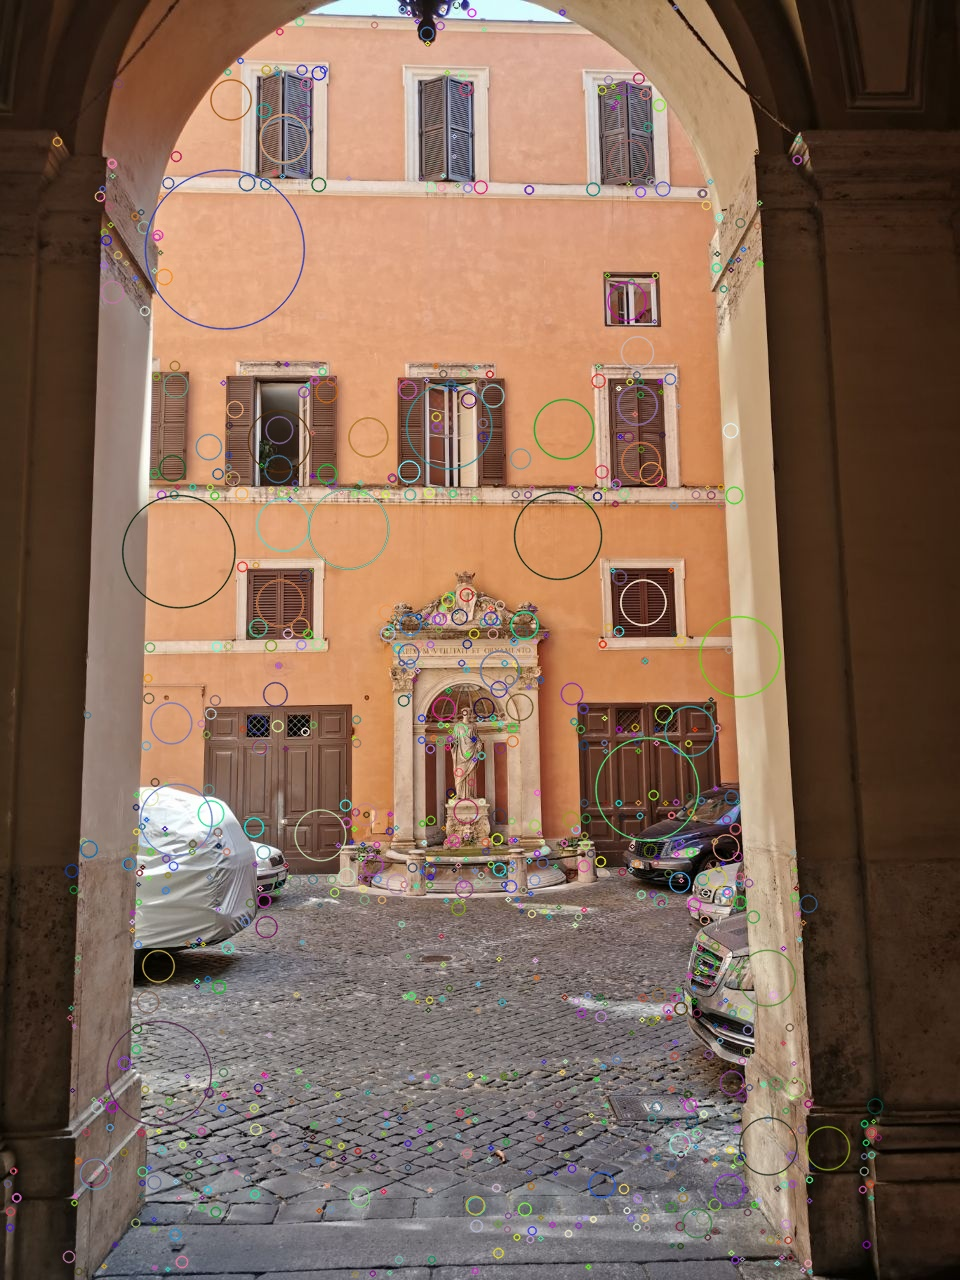
\includegraphics[scale=0.35,natwidth=960,natheight=1280]{10.jpg} 
	%\hfill
	%\includegraphics[scale=0.25,natwidth=684,natheight=912]{3.jpg} 
  \caption{An image with found blobs (denoted by circles) on it. The circles are centered at the blobs locations, sizes of circles correspond to the blobs sizes.}
  \label{fig:example2}
 \end{figure} 

Let us survey different interpretations of the blob detection algorithm, blobs and blob response functions. In \cite{blob} the author interpreted the algorithm by measuring its action on a model blob signal. In \cite{GenLapl, GenLaplNucl} the authors view steps of scale-space construction and blob response calculation as a one step of the Laplacian of Gaussian filters application. In \cite{VesselEnh} the authors used the multiscale Hessian in the image Taylor expansion as a characteristic term of an image surface. In \cite{CHEF} the trace and the determinant of the image multiscale Hessian are used as a sign of "ellipticity" of an image surface. In \cite{WaveMax} blobs are interpreted as extremum lines of an application of a wavelet. An article \cite{RectBlobs} provides an analysis of the blob detection action on a rectangular model of an ideal blob. In \cite{ColorBlob} it is said that inside a blob the Hessian matrix is the main characteristics of an image surface. In \cite{BlobCurv1} the multiscale Hessian determinant is used as an approximation of the image surface Gaussian curvature. In \cite{ColorBlob2} a convolution of the Laplacian of Gaussian is viewed as a change of brightness from a blob inner region toward a background. In \cite{LaplCurvCorn} the multiscale Laplacian of Gaussian is used for detecting of corners on a curve. In \cite{CornVertDet} there is an analysis of an application of the Hessian determinant and the Laplacian of Gaussian on the ideal corner model. The paper \cite{JuctionBlob} analyzes the behavior in the scale space of different junction models under the Laplacian of Gaussian operator. In the paper \cite{LinearBlob} the authors provide an interpretation of the blob response functions as quantities which measures how an image deviates from a linear function at a scale $t$. Though informally this interpretation is similar to ours, formal definitions are much different. Also the interpretation from \cite{LinearBlob} can't lead to the generalization of the algorithm to the non-scalar-valued case. In \cite{PhysicalBlob} blobs are interpreted as regions which are different from surroundings. In the paper \cite{DetHessExpMod} there is an analysis of blob detection applied to an ideal blob model. A blob is modeled by the multivariate exponential function. In \cite{BlobCurv2} the Hessian is interpreted as the second fundamental form of an image surface. In \cite{AtomicBlob} a sign of the Hessian determinant is used as a feature describing an image surface. The paper \cite{BrainMR} interprets the blob response functions as linear filters. In the paper \cite{LoGL0} a convolution of the Laplacian of Gaussian is also viewed as a change of brightness from a blob inner region toward a background. This interpretation allows the authors to define a new blob response function, which performs better than the Laplacian of Gaussian in low-contrast images and with irregular-shaped blobs.
\\
Our interpretations of the blob response functions are presented in the next chapters
\\
Implementation strategies and implementation details of the blob detection algorithm are discussed in the articles \cite{SIFT1, SIFT2, SURF, SpeedSIFT, SIFTImpl}.

\section{The problem introduction}

Consider the general case of an image being a map between manifolds $I(x):X \to Y$.  Let's look at the straightforward generalization of the blob detection stages:
\begin{enumerate}
\item Scale-space calculation. 
\\
$L(x,t)$ can be calculated as the solution of the manifold-valued heat equation, analogous to the scalar-valued case:
\begin{equation}\partderiv{L(x, t)}{t}=\tr H_L(x, t), L(x, 0)=I(x), \end{equation}.
where $H_L(x, t)$ is the covariant Hessian, the covariant differential of the differential: $H_L=\CovariantDiff \Diff L,H_L \in \CotangentBundle{X}\otimes\CotangentBundle{X}\otimes\TangentBundle{Y}$.
\\
Methods of the manifold-valued PDEs solution for different cases (in particular for the heat equation) are discussed in the papers \cite{Harmonic,Kimmel,ManifoldPDEClosest} and others. These methods are out of scope of our work.
\item Blob response calculation. 
\\
As the Hessian is not a matrix but a (2,1) tensor, the determinant blob response $BR_{\det}=t^n \det H_L$ is not defined and the trace blob response is a vector-valued function $BR_{\tr}=t \tr H_L \in \TangentBundle{Y}$. 
\item Blobs centers calculation. 
\\
The trace blob response is a vector-valued function: $BR_{\tr}=\tr{H_L} \in TY$. So we can find its extremums as extremums of a vector function or separately for each coordinate. In the first case the number of detected blobs will be too small, in the second case we disregard the correlation between different coordinates.
\end{enumerate} 

Let's review existing generalizations of the blob detection algorithm for non-scalar-valued cases (mainly for the color images) and see different approaches to the aforementioned generalization problems. Most of the approaches in one way or another reduce the problem to the scalar-valued case, mostly by projecting the vector-valued derivatives on some direction. 
\\
In \cite{ColorBlobRGB} vector-valued derivatives are substituted with their projections on a vector, defined by a color at a point. Similarly, in \cite{ColorBlob, ColorBlob2} vector-valued derivatives are projected on a vector, the vector is defined by the value of the scale-space Laplacian at a point. In \cite{ColorSIFT} a color invariant quantity is used as a scalar-valued input of the algorithm. In \cite{QuaternionColorCurv} a color vector is represented as the imaginary part of a quaternion, and the Quaternion SVD is used for the Hessian matrix. The drawback of this approach is that only vectors of dimension 3 can be processed. In \cite{ColorSURF} each color channel is simply processed separately, and then the results are combined. The drawback of this approach is that by this procedure correlations between different channels are disregarded. In the paper \cite{MRIBlob} the Di Zenzo gradient \cite{DiZenzo} (which is a vector) is used instead of a color image gradient (which is a matrix). With this substitution the Hessian becomes a matrix. Then the closest symmetric matrix is used instead of the Hessian. The drawback of this approach is that we need to substitute the actual Hessian matrix with the symmetric approximation. In the paper \cite{GROM} the following framework is proposed: 1) search of the “local optimal color”, 2) conversion of a local neighborhood from a multichannel image to a single-channel basis and 3) application of a single-channel detector in the local neighbourhood. The local optimal color is defined by using the scale-space Laplacian. In the article \cite{GA_SIFT} the geometric algebra is used as a representation of an image spectral information. Instead of usual scale-space calculation a two-side convolution with the geometric Gaussian is defined. The norm of the difference of the Gaussians is used as a blob response. A similar procedure is used in the work \cite{GA_SURF}, but the determinant of the Hessian is used as a blob response. Though the process of its computation is not clear from the article. In the article \cite{OnePCA} there is only one projection direction for the whole image, which is determined by PCA on the image color vectors. In our previous work \cite{RiemannianBlob} the blob response functions were defined for the manifold-valued case by means of image surface curvature. The drawback of this approach is that usage of curvatures was not clearly motivated from the algorithmic and intuitive heuristic point of view. Also scale normalization was not incorporated into the curvatures framework.
\\
Our key ideas about the generalization are the following:
\begin{enumerate}
\item The blob response functions should be interpreted as quantities showing a difference of an image at a scale $t$ from being linear. The idea of this interpretation is that a linear function is the most different from being a blob, because it has no difference with surroundings. So the more different is an image from being linear at a point, the more "blobness" it has.
\item These quantities should be easily extendable to the manifold case;
\item These quantities should remain scalar-valued in the manifold case.
\end{enumerate}
We present our approach in detail in the next chapter.

\section{Blob response functions as a difference from being linear}
Now let us present our interpretations of the blob response functions.

\begin{theorem} \label{SimpleInterp}
Let $f:\Rn \to \R$. Then:
\begin{multline*}BR_{\tr}(x_0, t) = t \tr H_f(x_0) = \\
 =\limeps \frac{1}{c_n \epsilon^2}
\int_{\| \delx \| = 1} (f - f_{lin})(x_0 + \sqrt{t}\epsilon \delx) d\delx, 
\end{multline*}
where $f_{lin}$ is the linear approximation of $f$ at a point $x_0$: $f_{lin}(x) = f(x_0) + df_{x_0}(x-x_0)$,
\\
$c_n$ is a constant depending on $n$.

\begin{multline*}|BR_{\det}(x_0, t)| = |t^n \det H_f(x_0)| = \\
 =\limeps \frac{
		\int_{tDf(\Ueps(x_0))} H_0 \big((tDf)^{-1}(y) \cap \Ueps(x_0) \big) dy} 
		{\Vol(\Ueps(x_0))}, \end{multline*}
where $Df:\Rn \to \Rn$ , $Df(x) = df_x$, i.e. to each point $x$ $Df$ appoints the differential of $f$ at this point,
\\
$H_0$ is a counting measure, i.e. it shows a number of elements in a set,
\\
$\Ueps(x_0)$ is an epsilon neighborhood of $x_0$,
\\
$H_0 \big((tDf)^{-1}(y) \cap \Ueps(x_0)$ is called the multiplicity function of $tDf(x)$.

\end{theorem}
Before the proof let us discuss the introduced equalities.
\\
We can see that the trace blob response $BR_{\tr}$ is equal to a difference of the function from the linear approximation over an infinitesimal neighborhood. The scale parameter $t$ corresponds to rescaling this neighborhood by $\sqrt{t}$ times. Note that $\sqrt{t}$ is a spatial scale of a Gaussian kernel which corresponds to the heat equation. So the trace blob response $BR_{\tr}$ can be viewed as a scale-normalized difference of the function from being linear.
\\
The absolute value of the determinant blob response $|BR_{\det}|$ is equal to the volume (taken with considerations of the multiplicity) of a set of gradient vectors of $f$ over an infinitesimal neighborhood. I.e. it can be viewed as a measure of diversity of the gradient of $f$. The scale parameter $t$ corresponds to rescaling of the gradient vectors by $t$. Taking into account that for a linear function this measure is equal to zero (as its gradient is constant), $|BR_{\det}|$ can be viewed as a scale-normalized measure of non-linearity.
\\
Let's prove the aforementioned interpretations. For the proof we will need the following Lemma.
\begin{lemma}  \label{BilinearFormTrace}
Let $B:\Rn \times \Rn \to \R$ be a symmetric bilinear form. Then 
$$\tr B = \frac{1} {c_n} \int_{\|x\|=1} B(x, x) dx,$$
where $c_n$ is a constant depending only on $n$.
\end{lemma} 

\begin{proof}
For the $B$ in major axes: $\int_{\|x\|=1} B(x, x) dx = \int_{\|x\|=1} \sum_i \lambda_i x_i^2 dx = \sum_i \lambda_i \int_{\|x\|=1} x_i^2 dx$.
The integral $\int_{\|x\|=1} dx$ is the integral over the unit sphere. As the sphere is symmetric, $\forall i, j \int_{\|x\|=1} x_i^2 dx = \int_{\|x\|=1} x_j^2 dx = c_n$. So $\int_{\|x\|=1} B(x, x) dx = \sum_i \lambda_i c_n = tr B c_n$ \qed
\end {proof}
Now return to the proof of the Theorem \ref{SimpleInterp}.
\begin{proof}
First, consider the trace blob response. Let's expand $f$ into the Taylor series: 
$$f(x_0 + \delx) = f(x_0) + df(\delx) + \frac{1}{2} H_f(\delx, \delx) + o(\|\delx \|^2),$$
$$\frac{1}{2} H_f(\delx, \delx) = f(x_0 + \delx) - ( f(x_0) + df(\delx) ) + o(\|\delx \|^2).$$
From the Lemma \ref{BilinearFormTrace}: 
$$t \tr H_f = \frac{1} {c_n} \int_{\|\delx\|=1} t H_f(\delx, \delx) d\delx = $$
$$ = \frac{1} {c_n} \int_{\|\delx\|=1} \frac{H_f(\epsilon \sqrt{t} \delx, \epsilon \sqrt{t} \delx)} {\epsilon^2} d\delx = $$
\begin{multline*} = \frac{2} {c_n \epsilon^2} \int_{\|\delx\|=1} f(x_0 + \epsilon \sqrt{t} \delx) - ( f(x_0) + df(\epsilon \sqrt{t} \delx) ) +
\\
+ o(\|\epsilon \sqrt{t} \delx \|^2) d\delx = \end{multline*}
$$ = \frac{2} {c_n \epsilon^2} \int_{\|\delx\|=1} (f-f_{lin})(x_0 + \epsilon \sqrt{t} \delx) d\delx + \frac{2}{c_n \epsilon^2}o(\epsilon^2). $$ 
Then put $\frac{1}{2}$ in $c_n$, take the limit with $\epsilon \to 0$, and we will obtain the first proposition of the Theorem \ref{SimpleInterp}.
\\
Then consider the determinant blob response $BR_{\det}$. Consider the area formula \cite{CartesianCurr} for the function $tDf$:
\begin{multline*}\int_{\Ueps(x_0)} J_{tDf}(x) dx = \\
= \int_{tDf(\Ueps(x_0))} H_0 \big((tDf)^{-1}(y)  \cap \Ueps(x_0)\big) dy,\end{multline*}
where $J_{tDf} = \sqrt{\det(\Diff tDf^* \Diff tDf)}$. For the function $tDf$ its differential $\Diff tDf(x) = t H_f(x)$. Then $J_{tDf} =$
\\
$= |t^n \det H_f|$ as $H_f$ is symmetric. Then
$$\int_{\Ueps(x_0)} J_{tDf}(x) dx = |t^n| \int_{\Ueps(x_0)} |\det H_f(x)| dx = $$
$$ = |t^n| \Big( \int_{\Ueps(x_0)} |\det H_f(x_0)| dx + \int_{\Ueps(x_0)} O(\epsilon) dx\Big) = $$
$$ = |t^n| \Vol(\Ueps(x_0)) |\det H_f(x_0)|  + \Vol(\Ueps(x_0)) O(\epsilon) dx.$$
Then 
\begin{multline*} |t^n \det H_f(x_0)| = 
\\
\frac{
		\int_{tDf(\Ueps(x_0))} H_0 \big((tDf)^{-1}(y) \cap \Ueps(x_0) \big) dy} 
		{\Vol(\Ueps(x_0))} + O(\epsilon).\end{multline*}
Take the limit with $\epsilon \to 0$ and obtain the second proposition of the Theorem \ref{SimpleInterp}. \qed
\end {proof}

\section{Notations and definitions}
Let us introduce some preliminary notations for a further discussion of the manifold case. These notations will be used in definitions, theorems and proofs till the end of the paper. The definitions of used differential geometric notions can be found in textbooks such as \cite{DiffGeom}.
\\
All functions here and further are considered to be smooth. All manifolds here and further are considered to be smooth, equipped with a connection without torsion and equipped with a metric.
\\
Let $X$ and $Y$ be manifolds, $\dim(X)=n, \dim(Y)=m$.

\begin{definition} \label{Affine}
A function $g:X \to Y$ is affine if it preserves the parallel transport \cite{GeodesicMaps}. In more detail, let a curve $\gamma(t): I \to X$ pass through $x_0$at $t = 0$. Let $u(t):I \to TX$ be a parallel tangent vector field on it such that $\CovariantDeriv{\dot{\gamma(0)}} u(t) = 0$ at $x_0$. Then $g$ is affine at $x_0$ if $\CovariantDeriv{\dot{g(\gamma)(0)}}$.
\end{definition}

\begin{definition} \label{CovariantHessian}
A covariant Hessian of a function $g:X \to Y$ is the covariant differential of its differential: $H_g \in \HessianSpace{X}{Y}:= \CovariantDiff dg$. The covariant differential of $dg$ is taken as the covariant differential of an element of $\DiffSpace{X}{Y}{g}$. 
\end{definition}
The covariant Hessian is also called the fundamental form of a map in literature. From \cite{GeodesicMaps} we know that for torsion-free connections the covariant Hessian is symmetric, and that $H_g = 0$ if and only if $g$ is affine. Further properties of the covariant Hessian are discussed in \cite{GeodesicMaps, RiemannianBlob}. We will call the covariant Hessian simply the Hessian when it will not cause any confusion.
\\
Let $f:X \to Y$ be a smooth function, $x_0 \in X, f(x_0) = y_0 \in Y$.
\\
Let $\{x_i\}$ be the normal coordinates centered at the point $x_0$, let $\{y_{\alpha}\}$ be the normal coordinates centered at the point $y_0$.
\\
$f_{\affine}(x_0 + \delx)=f(x_0) + \Diff f_{x_0}(\delx)$ in the aforementioned coordinates $\{x_i\}$ and $\{y_{\alpha}\}$. From the Taylor expansion at $x_0$ $f_{\affine}$ is the first-order approximation of $f$ at $x_0$. As we will see further $f_{\affine}$ is an affine function at the point $x_0$.
\\
Let $u, v \in Y$, $u, v$ are in the normal neighborhood of $y_0$. $\diff(u,v)$ is the following: take the geodesics $\gamma(t)$ from $u$ to $v$ in the natural parameter: $\gamma(0)=u, \gamma(s)=v$. Then $\diff(u, v)=\gamma'(0) dist(u, v)$.
\\
Let $\Gamma _y^{y_0}$ be the parallel transport map from the point $y$ to the point $y_0$ (in the corresponding bundles) along the geodesics connecting $y$ and $y_0$.
\\
Let $\diff^{\Gamma^{y_0}}(u, v) = \Gamma _u^{y_0}(\diff(u, v))$.
\\
Let $Df$ be a section of the vector bundle $TX \otimes TY$ which appoints to every point $x \in X$ the differential of $f(x)$ $\Diff f$.
\\
Let $Df^{\Gamma^{x_0}}(x):X \to T_{x_0}X \otimes T_{y_0}Y = \Gamma _x^{x_0}(Df(x))$.

\section{Definitions of the blob response in the manifold case}
In order to generalize the blob response functions to the manifold case, we will use the expressions, obtained in the previous chapter, as the definitions of the blob response functions. In order to use them in the manifold case, we should do a few modifications in them. Let us discuss these modifications before the formal statements of the blob response.
\\
First, there are no linear functions in the manifold case. As we said previously, instead of the linear functions we use affine functions. These are the mappings between manifolds which preserve the parallel transport. These functions will be described in more detail later. So in the definition of $BR_{\tr}$ instead of the linear approximation $f_{lin}$ we will use the affine approximation $f_{\affine}$. A proof that $f_{\affine}$ is indeed an affine function will be given later.
\\
Second, we can't subtract points on a manifold. We need some sort of "signed distance" between points in order to substitute it for subtraction. For this we take the velocity vector of the geodesics between points multiplied by the distance between the points. Then, as we need to integrate the obtained vectors, we should have them in the same fiber of $\TangentBundle{Y}$. For this we move these vectors by the parallel transport to the $\TangentSpaceArg{Y}{y_0}$.
\\
Third, if we want to calculate the volume of the differential tensors set in a neighborhood of $x_0$, these tensors should also belong to the same fiber of the corresponding tensor bundle. In order to provide this, we move the differential tensors by the parallel transport to the fiber of the point $x_0$.
\\
Then proceed to the formal definitions. 

\begin{definition} \label{ManifoldBlobResponse}
The trace manifold blob response is defined as:
\begin{multline*}BR_{\tr}^{\manifold}(x_0, t) = \\
=\|\limeps \frac{1}{c_n \epsilon^2}  
 \int_{\| \delx \| = 1} \diff^{\Gamma^{y_0}}(f(x), f_{\affine}(x)) d\delx \|,
\end{multline*}
where $x=x_0 + \sqrt{t}\epsilon \delx$.
\\
The determinant manifold blob response is defined as:
\begin{multline*}BR_{\det}^{\manifold}(x_0, t) = \\
 =\limeps \frac{
		\int_{tDf^{\Gamma^{x_0}}(\Ueps(x_0))} H_0 \big((tDf^{\Gamma^{x_0}})^{-1}(y) \cap \Ueps(x_0) \big) dy} 
		{\Vol(\Ueps(x_0))}. \end{multline*}

\end{definition}
Note that if $X=\Rn, Y=\R$ then 
$$BR_{\tr}^{\manifold} = |BR_{\tr}|, BR_{\det}^{\manifold} = |BR_{\det}|.$$

Next we should motivate the introduced definitions. First, we need to show that the class of the affine functions is a good substitution for the linear functions from the point of view of the blob detection algorithm understanding. I.e. that the affine functions still possess the property of "not being different from surroundings". Second, we need to show that $f_{\affine}$ is indeed an affine function. Third, we need to show that the volume of the differentials set (in the determinant manifold blob response definition) can still be viewed as a measure of a difference from being affine. 
\\
In order to answer these requests we need the following lemmas:

\begin{lemma}\label{HessianCoordinate}
Let $f:X \to Y$. Let $\{x_i\}$ be normal coordinates on $X$ centered at $x_0$, $\{y_{\alpha}\}$ be normal coordinates on $Y$ centered at $f(x_0)$. Let $H_f$ be a covariant Hessian of $f$, i.e. a covariant differential of $df$ as an element of $\DiffSpace{X}{Y}{f}$. Then in these coordinates
$$H_f(x_0)_{ij}^{\alpha} = \frac{\partial^2 f^{\alpha}}{\partial x_i \partial x_j},$$
i.e. in the normal coordinates the covariant hessian coincides with the coordinate hessian.
\end{lemma}

\begin{proof}
From \cite{RiemannianBlob} Proposition 1: 
$$H_f(u, v) = \CovariantDerivManif{\TPreimage{Y}{f}}{v}(df(u)) - df(\CovariantDeriv{v}u).$$
Then the coordinate expression is the following: 
$$H_f(e_i, e_j)^{\alpha} = \frac{\partial^2 f^{\alpha}}{\partial x_i \partial x_j} + \Gamma^{\TPreimage{Y}{f}\alpha}_{jl}df(e_i)^l - df(\Gamma^k_{ij}e_k)^{\alpha}.$$
The third term is zero in the normal coordinates $\{x_i\}$. Let's review the second term. From the equality of the connection forms $\omega^{i\TPreimage{Y}{f}}_j = f^*\omega^{i Y}_j$ we conclude that $\Gamma^{i\TPreimage{Y}{f}}_{kj}=\Gamma^{iY}_{lj}df^l_k = 0$ in the normal coordinates $\{y_{\alpha}\}$. Hence 
$H_f(e_i, e_j)^{\alpha} = \frac{\partial^2 f^{\alpha}}{\partial x_i \partial x_j}$. \qed
\end{proof}

\begin{lemma}\label{AffineLinear}
Let $g:X \to Y$. Let $\{x_i\}$ be normal coordinates on $X$ centered at $x_0$, $\{y_{\alpha}\}$ be normal coordinates on $Y$ centered at $g(x_0)$. Then $g$ is affine if and only if $g$ has a linear coordinate form, i.e. $g(x) = Ax$, where $A$ is a matrix, in the coordinates $\{x_i\}$, $\{y_{\alpha}\}$.
\end{lemma}

\begin{proof}
By \cite{GeodesicMaps} $g$ is affine if and only if $H_g = 0$. By Lemma \ref{HessianCoordinate} ${H_g}_{ij} = \frac{\partial^2 g^{\alpha}}{\partial x_i \partial x_j}$ in the coordinates  $\{x_i\}$, $\{y_{\alpha}\}$, so $H_g = 0$ if and only if $g$ has a linear coordinate form. \qed
\end{proof}

The above lemma give answer to the second request. Indeed, $f_{\affine}(x_0 + \delx)=f(x_0) + \Diff f_{x_0}(\delx)$ has a linear coordinate form in the normal coordinates so it is an affine mapping.
\\
The following proposition gives the answer to the first request. The proposition states that the graph of an affine function $g:X\to Y$ can be viewed as "consisting of geodesics" of the ambient space $X \times Y$ at the point $x_0, g(x_0)$. So we can say that the function $g(x)$ has no difference with surroundings, as in the linear function case.

\begin{proposition} \label{AffineCurv}
Let $g:X\to Y$ be an affine at the point $x_0$. Let $Gr_g$ be a graph of $g$, immersed in $X \times Y$. Let $\tilde{g}:X\to X \times Y = (x, g(x))$. Let $\gamma(t)$ be a geodesics on $X$, passing through the point $x_0$. Then the curve $\tilde{g}(\gamma(t))$ is a geodesics of $X \times Y$.
\end{proposition}
\begin{proof}
In the normal coordinates $\{x_i\}, \{y_{\alpha}\}$ 
$$\tilde{g}(x)= \begin{cases} 
      x_i = x_i \\
      y_{\alpha} = \sum a_{{\alpha}j} x_j 
   \end{cases}$$
By the Lemma \ref{AffineLinear} $\tilde{g}$ is an affine map, so it preserves the parallel transport. Also it is a diffeomorphism, so it maps curves into curves. By these observations we conclude that $\tilde{g}$ maps geodesics, passing through $x_0$ for the geodesics, passing through $(x_0, g(x_0))$. \qed
\end{proof}

The answer to the third request is given by the one of the properties of the affine functions. It states that the covariant derivative of the differential of an affine function is zero in every direction \cite{GeodesicMaps}. So the differential of an affine at the point $x_0$ function is constant in an infinitesimal neighborhood of $x_0$. Thus the volume of the set of the differentials (from the determinant manifold blob response definition) can be viewed as a measure of a difference from being an affine.

\section{Expressions of the manifold blob response through the Hessian}
The drawback of the introduced definitions of the manifold blob response is that they are not computationally tractable. If we want to implement the algorithm we need to express the definitions through some quantities which we can compute. For this we express the manifold blob response functions through the Hessian. The formal statements are given in the next theorems. 
\begin{theorem}\label{BR_trHess}
$$BR_{\tr}^{\manifold}(x,t)=t\|\tr H\|,$$
where $H$ is the covariant Hessian of $f$, $H \in \HessianSpace{X}{Y}$,
\\
$\|\|$ is a norm in $T_{y_0} Y$.
\end{theorem}

\begin{theorem}\label{BR_detHess}
$$BR_{\det}^{\manifold}(x,t)=t^n\sqrt{\det (\sum_{i=1}^{m} H^i H^i)},$$
where $H$ is the covariant Hessian of $f$, $H \in \HessianSpace{X}{Y}$,
\\
$H^i = (h_{kl}^i)_{1 \le k,l \le n}$, i.e. it is a component of the Hessian which corresponds to the $i$th coordinate of $T_{y_0} Y$.
\end{theorem}

For the proof we will need the following lemmas.

\begin{lemma}\label{ParallelTransport}
Let $x \in \Ueps(x_0)$. Let $(\bigeps, \pi, X)$ be a vector bundle over $X$, $\dim\bigeps=m$. Let $\{x_i, u_\alpha\}$ be such coordinates over $\bigeps$ that $\{x_i\}$ are normal coordinates on $X$ centered at the point $x_0$ and that $\Gamma^{i\bigeps}_{jk}(x_0) = 0 \forall i,j,k$. Let $a \in \pi^{-1}(x)$. Then
$$\Gamma_x^{x_0}(a)^i - a^i = O(\epsilon^2)|a^i|,$$
where all operations in the formula are done over the coordinate expressions of the vectors.
\end{lemma}

\begin{proof}
Write down the parallel transport equations:
$$a^i(s) = a^i(0) - \int_0^s \Gamma^{i\bigeps}_{kj}(x(t)) \dot{x}^k(t)a^j(t) dt.$$
As $\{x_i\}$ are normal coordinates, $t \le s = dist(x, x_0) \le \epsilon$. $\Gamma^{i\bigeps}_{kj}(t) = \dot{\Gamma}^{i\bigeps}_{kj}(0) + r_1(t)$, where $r_1(t)=o(t)$. Then $|\Gamma^{i\bigeps}_{kj}(t)| \le C_1 t + r_1^{max}$. $|\dot{x}^k(t)| \le C_2$, $|a^j(t)| \le C_3$. So
$$|a^i(s) - a^i(0)| \le \int_0^s (C_1 t + r_1^{max})C_2 C_3 dt = o(\epsilon).$$
So $|a^i(t)| = |a^i(0)| + r_2(t)$, where $r_2(t)=o(\epsilon)$. Then $|a^i(t)| \le |a^i(0)| + r_2^{max}$. Substitute this into the equation:
\begin{multline*}|a^i(s) - a^i(0)| \le \int_0^s (C_1 t + r_1^{max})C_2 (|a^i(0)| + r_2^{max}) dt = \\
= |a^i(0)| O(\epsilon ^2)\end{multline*} \qed
\end{proof}

\begin{lemma} \label{ChristoffelSymbolsDiffSpace}
Let $f:X\to Y$. Let $\{x_i\}$ be normal coordinates centered at the point $x_0 \in X$, $\{y_{\alpha}\}$ be normal coordinates centered at the point $f(x_0) \in Y$. Then for the vector bundle $\DiffSpace{X}{Y}{f}$ the Christoffel symbols $\Gamma^k_{ij}=0, 1 \le i \le n, 1 \le k,j \le mn$ in the induced coordinates.
\end{lemma}
\begin{proof}
If we apply the covariant differentiation Leibnitz rule to the definition of the Christoffel symbols of $\DiffSpace{X}{Y}{f}$, we will obtain that they are a linear combination of the Christoffel symbols of $X$ at $x_0$ and of $Y$ at $f(x_0)$. As the Christoffel symbols of $X$ and $Y$ are zero in the normal coordinates, then the Christoffel symbols of $\DiffSpace{X}{Y}{f}$ are also zero in the induced coordinates at the point $x_0$. \qed
\end{proof}

Then return to the Theorem \ref{BR_trHess}.
\begin{proof}
Let $\gamma(l):\R \to Y, \gamma(0) = f(x), \gamma(s) = f(x_0) + df_{x_0}(\sqrt{t}\epsilon\delx)$ be a geodesics in the natural parameter, where $x=x_0 + \sqrt{t}\epsilon\delx$. Let $dist = dist(f(x), f(x_0) + df_{x_0}(\sqrt{t}\epsilon\delx))$. Then $\diff^{\Gamma^{y_0}}(f(x), f_{\affine}(x)) =$ \\
$ = \Gamma_y^{y_0}(\dot{\gamma}(0)) dist =$ (from the Lemma \ref{ParallelTransport}) $=(\dot{\gamma}(0) + O(dist^2)|\dot{\gamma}(0)|) dist$. Then 
\begin{multline*}
\frac{1}{c_n \epsilon^2} \int_{\| \delx \| = 1} \diff^{\Gamma^{y_0}}(f(x), f_{\affine}(x)) d\delx = \\
= \frac{1}{c_n \epsilon^2} \int_{\| \delx \| = 1} \dot{\gamma}(0) dist + O(dist^3) d\delx.
\end{multline*}
Let's review the first term. Expand $\gamma(l)$ into the Taylor series:
$$f(x) = f(x_0) + df_{x_0}(\sqrt{t}\epsilon\delx) + \dot{\gamma}(0)dist + o(dist).$$ 
So $\dot{\gamma}(0)dist = f(x) - (f(x_0) + df_{x_0}(\sqrt{t}\epsilon\delx))  + o(dist)$. Substitute this into the above integral and obtain
\begin{multline*}\frac{1}{c_n \epsilon^2} \int_{\| \delx \| = 1} \big( f(x) - (f(x_0) + df_{x_0}(\sqrt{t}\epsilon\delx)) + \\
+ o(dist) + O(dist^3)\big) d\delx.\end{multline*}
Then expand $f$ into the Taylor series:
\begin{multline*}f(x) = f(x_0) + df_{x_0}(\sqrt{t}\epsilon\delx) + \\
+ \frac{1}{2} H_{coord} (\sqrt{t}\epsilon\delx, \sqrt{t}\epsilon\delx) + o(\epsilon^2),\end{multline*}
where ${H_{coord}}_{ij}^{\alpha} = \frac{\partial^2 f^{\alpha}}{\partial x_i \partial x_j}$. Substitute this into the integral and obtain:
\begin{multline*}\frac{1}{2 c_n \epsilon^2} \int_{\| \delx \| = 1} \big( H_{coord} (\sqrt{t}\epsilon\delx, \sqrt{t}\epsilon\delx) + \\
+ o(\epsilon^2) + O(dist^3)\big) d\delx. \end{multline*}
Then express $dist$ through $\epsilon$. From the Taylor expansion of $\gamma$: $dist = O\big(f(x) - (f(x_0) + df_{x_0}(\sqrt{t}\epsilon\delx))\big) = O(H_{coord}(\sqrt{t}\epsilon\delx, \sqrt{t}\epsilon\delx) + o(\epsilon^2)) = O(\epsilon^2)$. Hence $O(dist^3) = o(\epsilon^2)$. Substitute this into the integral, take the limit $\epsilon \to 0$, apply the Lemma \ref{BilinearFormTrace} and obtain: $BR_{\tr}(x_0, t) = t\|\tr H_{coord} \|$. This equality is achieved in the normal coordinates $\{x_i\}, \{y_{\alpha}\}$, because $\|\tr H_{coord} \|$ is coordinate-dependent since $H_{coord}$ is not a tensor. In these coordinates (from the Lemma \ref{HessianCoordinate}) $H_{coord} = H$, where $H$ is the covariant Hessian. Since $H$ is a tensor, $\|\tr H \|$ is coordinate-independent. So $BR_{\tr}(x_0, t) = t\|\tr H \|$ in all coordinate systems, because all parts of equality are coordinate-independent. \qed
\end{proof}
Then let's prove the Theorem \ref{BR_detHess}.
\begin{proof}
We want to apply the area formula to the numerator of the determinant blob response definition. In order to do this let's find the differential of $tDf^{\Gamma^{x_0}}$ at the point $x_0$. Write down the parallel transport equation for $tDf$ and differentiate it:
$$\frac{\partial (tDf^{\Gamma^{x_0}})^i}{\partial x_j} = \frac{\partial (tdf^i)}{\partial x_j} 
+ \frac{\partial \Big(\int_0^s \Gamma^i_{jk}(x(l))\dot{x^k}(l)a^j(l)dl\Big)}{\partial x_j},$$
where $df$ is viewed as a row-vector.
Find out the second term by the definition of the derivative at the point $x_0$. Let $r(x) = \int_0^{s(x)} \Gamma^i_{jk}(x(l))\dot{x^k}(l)a^j(l)dl$. Then
\begin{multline*} \lim_{x \to x_0} \frac{r(x) - r(x_0)}{x - x_0} = \\
= \lim_{x \to x_0} \frac{\int_0^s \Gamma^i_{jk}(x(l))\dot{x^k}(l)a^j(l)dl - 0}{x - x_0} = \\
= \textrm{(by the Lemmas \ref{ParallelTransport} and \ref{ChristoffelSymbolsDiffSpace})} \lim_{x \to x_0} \frac{df^i O \big((x-x_0)^2 \big)}{x-x_0} = 0.
\end{multline*} 
So in the normal coordinates the differential of $tDf^{\Gamma^{x_0}}$ at the point $x_0$ has the coordinates $\frac{\partial (tdf^l)}{\partial x_j} = t\frac{\partial^2 f^{\alpha}}{\partial x_i \partial x_j}$. From the Lemma \ref{HessianCoordinate} it has the same matrix as the covariant Hessian at the point $x_0$ multiplied by $t$. Also they are the elements of the same tensor space: at the point $x_0$ they both belong to $\CotangentSpaceArg{X}{x_0}\otimes \CotangentSpaceArg{X}{x_0}\otimes \TArgPreimage{Y}{y_0}{f}$. From this it follows that they are equal. Then the Jacobian of $tDf^{\Gamma^{x_0}}$ is equal to
$t^n\sqrt{\det (\sum_{i=1}^{m} H^i H^i)}$. Substitute it into the area formula, and after mild transformations obtain :
\begin{multline*} t^n\sqrt{\det (\sum_{i=1}^{m} H^i H^i)} = 
\\
\frac{
		\int_{tDf^{\Gamma^{x_0}}(\Ueps(x_0))} H_0 \big((tDf^{\Gamma^{x_0}})^{-1}(y) \cap \Ueps(x_0) \big) dy} 
		{\Vol(\Ueps(x_0))} + O(\epsilon).\end{multline*}
Take the limit with $\epsilon \to 0$ and obtain the proposition of the theorem. \qed
\end{proof}
%\begin{acknowledgements}
%If you'd like to thank anyone, place your comments here
%and remove the percent signs.
%\end{acknowledgements}


% Authors must disclose all relationships or interests that 
% could have direct or potential influence or impart bias on 
% the work: 
%
% \section*{Conflict of interest}
%
% The authors declare that they have no conflict of interest.


% BibTeX users please use one of
%\bibliographystyle{spbasic}      % basic style, author-year citations
%\bibliographystyle{spmpsci}      % mathematics and physical sciences
%\bibliographystyle{spphys}       % APS-like style for physics
%\bibliography{}   % name your BibTeX data base

% Non-BibTeX users please use
\begin{thebibliography}{16}
%
\bibitem{CircleData1}
J. Bioucas-Dias, V. Katkovnik, J. Astola, and K. Egiazarian: 
Absolute phase estimation: adaptive local denoising and global unwrapping, 
Applied Optics, 47 (2008), pp. 5358–5369.

\bibitem{CircleData2}
C.-A. Deledalle, L. Denis, and F. Tupin:
NL-InSAR: Nonlocal interferogram estimation, 
IEEE Transactions on Geoscience Remote Sensing, 49 (2011), pp. 1441–1452.

\bibitem{CircleData3}
R. Bergmann, F. Laus, G. Steidl, and A. Weinmann: 
Second order differences of cyclic data and applications in variational denoising,
SIAM Journal on Imaging Sciences, 7 (2014), pp. 2916–2953.

\bibitem{SphereData1}
R. Kimmel and N. Sochen:
Orientation diffusion or how to comb a porcupine, 
Journal of Visual Communication and Image Representation, 13 (2002), pp. 238–248.

\bibitem{SphereData2}
L. A. Vese and S. J. Osher:
Numerical methods for p-harmonic flows and applications to image processing,
SIAM Journal on Numerical Analysis, 40 (2002), pp. 2085–2104.

\bibitem{SphereData3}
T. F. Chan, S. Kang, and J. Shen:
Total variation denoising and enhancement of color images based on the CB and HSV color models
Journal of Visual Communication and Image Representation, 12 (2001), pp. 422–435.

\bibitem{SO3Data1}
F. Bachmann, R. Hielscher, and H. Schaeben:
Grain detection from 2d and 3d EBSD data - Specification of the MTEX algorithm
Ultramicroscopy, 111 (2011), pp. 1720–1733.

\bibitem{SO3Data2}
R. Bergmann, R. H. Chan, R. Hielscher, J. Persch, and G. Steidl:
Restoration of manifold-valued images by half-quadratic minimization,
Inverse Problems in Imaging, 10 (2016), pp. 281–304.

\bibitem{SPDMatrixData1}
C. Chefd’Hotel, D. Tschumperle, R. Deriche, and O. Faugeras:
Regularizing flows for constrained matrix-valued images, 
Journal of Mathematical Imaging and Vision, 20 (2004), pp. 147–162.

\bibitem{SPDMatrixData2}
P. T. Fletcher and S. J.:
Principal geodesic analysis on symmetric spaces: Statistics of diffusion tensors, 
in Computer Vision and Mathematical Methods in Medical and Biomedical Image Analysis, vol. 3117, Springer, 2004, pp. 87–98.

\bibitem{SPDMatrixData3}
O. Tuzel, F. Porikli, and P. Meer:
Learning on Lie groups for invariant detection and tracking,
in CVPR 2008, IEEE, 2008, pp. 1–8.

\bibitem{blob}
Lindeberg, T.:
Feature detection with automatic scale selection. 
International journal of computer vision, 30(2), 79--116 (1998)

\bibitem{GenLapl}
Hui Kong, Hatice Cinar Akakin, Sanjay E. Sarma:
A Generalized Laplacian of Gaussian Filter for Blob Detection and Its Applications. 
IEEE Transactions on Cybernetics, 43, 6 , 1719--1733 (2013, December)

\bibitem{GenLaplNucl}
Hongming Xu, Cheng Lu, Richard Berendt, Naresh Jha, Mrinal Mandal:
Automatic Nuclei Detection Based on Generalized Laplacian of Gaussian Filters.
IEEE Journal of Biomedical and Health Informatics,21, 3, 826--837 (2017, May)

\bibitem{VesselEnh}
Alejandro F. Frangi, Wiro J. Niessen, Koen L. Vincken, Max A. Viergever:
Multiscale vessel enhancement filtering.
In: Wells W.M., Colchester A., Delp S. (eds) Medical Image Computing and Computer-Assisted Intervention — MICCAI’98. MICCAI 1998. Lecture Notes in Computer Science, vol 1496. Springer, Berlin, Heidelberg

\bibitem {CHEF}
Qing Yang, Parvin, B.:
CHEF: convex hull of elliptic features for 3D blob detection.
Pattern Recognition. Proceedings. 16th International Conference on, Volume: 2 (2002)

\bibitem {WaveMax}
Damerval, C., Meignen, S.:
Blob Detection With Wavelet Maxima Lines.
IEEE Signal Processing Letters, Volume: 14, Issue: 1 , pp. 39--42 (Jan. 2007)

\bibitem {RectBlobs}
Hinz, S.:
Fast and subpixel precise blob detection and attribution.
Image Processing, 2005. ICIP 2005. IEEE International Conference on, Volume: 3 (2005)

\bibitem {ColorBlob}
Khanina, N. A., Semeikina, E. V., Yurin, D. V.:
Scale-space color blob and ridge detection. 
Pattern Recognition and Image Analysis, 22(1), 221--227 (2012)

\bibitem {BlobCurv1}
Ferraz, L., Binefa, X.:
A sparse curvature-based detector of affine invariant blobs. 
Computer Vision and Image Understanding, 116(4), 524--537 (2012)

\bibitem {ColorBlob2}
Khanina, N.A., Semeikina, E.V.,Yurin:
Color Blob and line detection in scale-space.
D.V. Pattern Recognit. Image Anal.  21: 267, pp 267–269 (2011)

\bibitem {LaplCurvCorn}
Xiaohong Zhang, Ying Qu, Dan Yang, Hongxing Wang, Jeff Kymer:
Laplacian Scale-Space Behavior of Planar Curve Corners.
IEEE Transactions on Pattern Analysis and Machine Intelligence, Volume: 37, Issue: 11, pp.2207--2217 (Nov. 1 2015 )

\bibitem {CornVertDet}
Rachid Deriche, Gerard Giraudon:
A computational approach for corner and vertex detection.
Int J Comput Vision, pp. 101--124 (1993)

\bibitem {JuctionBlob}
S. A. Tabbone, L. Alonso, D. Ziou:
Behavior of the Laplacian of Gaussian Extrema.
J Math Imaging Vis, pp. 107–128 (2005)

\bibitem {LinearBlob}
Triet M. Le , Luke Rogers:
Detecting stable scales in images via non-smooth K-functionals.
UCLA CAM Report 10-63

\bibitem {PhysicalBlob}
Guyue Zhang, Jun Liu, Ye Liu, Jingwen Zhao, Luchao Tian, and Yan Qiu Chen:
Physical blob detector and Multi-Channel Color Shape Descriptor for human detection. 
J. Vis. Comun. Image Represent. 52, C, pp. 13--23. (April 2018)

\bibitem {DetHessExpMod}
Xu X.:
Blob Detection with the Determinant of the Hessian.
In: Li S., Liu C., Wang Y. (eds) Pattern Recognition. CCPR 2014. Communications in Computer and Information Science, vol 483. Springer, Berlin, Heidelberg

\bibitem {BlobCurv2}
Ferraz, L., Binefa, X.:
A scale invariant interest point detector for discriminative blob detection. 
In Iberian Conference on Pattern Recognition and Image Analysis, 233--240  (2009, June)

\bibitem {AtomicBlob}
Brendan P. Marsh, Nagaraju Chada, Raghavendar Reddy Sanganna Gari, Krishna P. Sigdel, Gavin M. King:
The Hessian Blob Algorithm: Precise Particle Detection in Atomic Force Microscopy Imagery.
Scientific Reports volume 8, Article number: 978 (2018) 

\bibitem {BrainMR}
Qolamreza R. Razlighi, Yaakov Stern:
Blob-like Feature Extraction and Matching for Brain MR Images.
Conf Proc IEEE Eng Med Biol Soc. 2011, pp. 7799--7802. (2011) 

\bibitem {LoGL0}
Zhenwei Miao ; Xudong Jiang ; Kim-Hui Yap:
Contrast Invariant Interest Point Detection by Zero-Norm LoG Filter.
IEEE Transactions on Image Processing, Volume: 25, Issue: 1, pp.331--342 (Jan. 2016)

\bibitem {SIFT1}
Lowe, David G.:
Object recognition from local scale-invariant features. 
Proceedings of the International Conference on Computer Vision. 2. pp. 1150--1157 (1999)

\bibitem {SIFT2}
Lowe, David G.:
Distinctive Image Features from Scale-Invariant Keypoints.
International Journal of Computer Vision. 60 (2): 91--110 (2004)

\bibitem {SURF}
Bay, H., Tuytelaars, T., Van Gool, L.:
SURF: Speeded Up Robust Features.
Proceedings of the ninth European Conference on Computer Vision (May 2006)

\bibitem {SpeedSIFT}
Grabner M., Grabner H., Bischof H.:
Fast Approximated SIFT. 
In: Narayanan P.J., Nayar S.K., Shum HY. (eds) Computer Vision -- ACCV 2006. ACCV 2006. Lecture Notes in Computer Science, vol 3851. (2006) 

\bibitem {SIFTImpl}
Rey-Otero, I., Morel, JM., Delbracio:
An Analysis of the Factors Affecting Keypoint Stability in Scale-Space
M. J Math Imaging Vis 56: 554 (2016) 


\bibitem {Harmonic}
Mémoli, F., Sapiro, G., Osher, S.:
Solving variational problems and partial differential equations mapping into general target manifolds. 
Journal of Computational Physics, 195(1), 263--292 (2004)

\bibitem {ManifoldPDEClosest}
Nathan D.King, Steven J.Ruuth:
Solving variational problems and partial differential equations that map between manifolds via the closest point method.
Journal of Computational Physics, Volume 336, pp. 330--346 (May 2017)


\bibitem {Kimmel}
Sochen, N., Kimmel, R., Malladi, R.: 
A general framework for low level vision. 
IEEE transactions on image processing, 7(3), 310--318 (1998)

\bibitem {ColorBlobRGB}
Anlong Ming, Huadong Ma:
A blob detector in color images.
CIVR '07 Proceedings of the 6th ACM international conference on Image and video retrieval, pp. 364--370 (2007)

\bibitem {ColorSIFT}
A.E. Abdel-Hakim ; A.A. Farag:
CSIFT: A SIFT Descriptor with Color Invariant Characteristics.
2006 IEEE Computer Society Conference on Computer Vision and Pattern Recognition (CVPR'06)

\bibitem {QuaternionColorCurv}
Shi, Lilong; Funt, Brian; Hamarneh, Ghassan: 
Quaternion Color Curvature. 
Final Program and Proceedings - IS and T/SID Color Imaging Conference. pp. 338--341. (2008).

\bibitem {ColorSURF}
Gossow, David; Decker, Peter; Paulus, Dietrich:
Extending Surf to the Color Domain
Conference on Colour in Graphics, Imaging, and Vision, CGIV 2010 Final Program and Proceedings, pp. 215--221(7)

\bibitem {MRIBlob}
K. Krishna Nand,Rafeef Abugharbieh, Brian G. Booth, Ghassan Hamarneh:
Detecting Structure in Diffusion Tensor MR Images.
Fichtinger G., Martel A., Peters T. (eds) Medical Image Computing and Computer-Assisted Intervention – MICCAI 2011. MICCAI 2011. Lecture Notes in Computer Science, vol 6892 (2011)

\bibitem {DiZenzo}
Silvano Di Zenzo:
A note on the gradient of a multi-image.
Computer Vision, Graphics, and Image Processing, Volume 33, Issue 1, pp. 116--125 (January 1986)


\bibitem {GROM}
Smirnov, P., Semenov, P., Lyakh, M., Chun, A., Gusev, D., Redkin, A., Srinivasan, S.:
GRoM --- Generalized robust multichannel feature detector. 
In Signal and Image Processing Applications, 2011 IEEE International Conference on, 585--590 (2011, November)

\bibitem {GA_SIFT}
Y. Li et al.: 
GA-SIFT: A new scale invariant feature transform for multispectral image using geometric algebra.
Inform. Sci. (2014)

\bibitem {GA_SURF}
Wang, R., Shi, Y., Cao, W.:
GA-SURF: A New Speeded-Up Robust Feature Extraction Algorithm for Multispectral Images Based on Geometric Algebra. 
Pattern Recognition Letters (2018)

\bibitem {OnePCA}
Stottinger, Julian; Hanbury, Allan; Gevers, T.; Sebe, Nicu.: 
Lonely but attractive: Sparse color salient points for object retrieval and categorization. 
2009 IEEE Conference on Computer Vision and Pattern Recognition, CVPR 2009. 1 - 8. 

\bibitem {RiemannianBlob}
Shestov, Aleksei; Kumskov, Mikhail: 
A Riemanian Approach to Blob Detection in Manifold-Valued Images. 
Geometric Science of Information: Third International Conference, GSI 2017, pp. 727--735. (2017)

\bibitem {CartesianCurr}
Giaquinta, Mariano; Modica, Giuseppe; Soucek, Jiri:
Cartesian Currents in the Calculus of Variations I.
Ergebnisse der Mathematik und ihrer Grenzgebiete. 3. Folge / A Series of Modern Surveys in Mathematics, 37 (1998)

\bibitem {GeodesicMaps}
Jaak Vilms:
Totally geodesic maps.
J. Differential Geom. 4 (1970), no. 1, 73--79.

\bibitem {Saucan}
Saucan, E., Wolansky, G., Appleboim, E., Zeevi, Y. Y.:
Combinatorial ricci curvature and laplacians for image processing. 
In Image and Signal Processing, CISP'09, 2nd International Congress on, 1--6 (2009)

\bibitem {Batard}
Batard, T., Berthier, M.:
Spinor Fourier transform for image processing. 
IEEE Journal of Selected Topics in Signal Processing, 7(4), 605--613 (2013)

\bibitem {ScalarBlob3D}
Zaharescu, A., Boyer, E., Varanasi, K., Horaud, R.:
Surface feature detection and description with applications to mesh matching. 
In Computer Vision and Pattern Recognition, 2009, 373--380 (2009, June)



\bibitem {DiffGeom}
Spivak, M.: 
Comprehensive introduction to differential geometry.
Vol. IV A (1981)

\bibitem {qsar}
Baskin, I., Varnek, I.:
Fragment Descriptors in SAR/QSAR/QSPR Studies, Molecular Similarity Analysis and in Virtual Screening.
Chemoinformatic Approaches to Virtual Screening, 1--43 (2008)

\bibitem {molecular}
Connolly, M. L.:
Analytical molecular surface calculation. 
Journal of Applied Crystallography, 16(5), 548--558 (1983)

\bibitem {bag}
Csurka, G., Dance, C., Fan, L., Willamowski, J., Bray, C.: 
Visual categorization with bags of keypoints. 
In Workshop on statistical learning in computer vision, ECCV, Vol. 1, No. 1-22, 1--2 (2004, May). 

\bibitem {cross}
Kohavi, R.:
A study of cross-validation and bootstrap for accuracy estimation and model selection. 
In Ijcai, Vol. 14, No. 2, 1137--1145 (1995, August)

\bibitem {SVM}
Weston, J., Mukherjee, S., Chapelle, O., Pontil, M., Poggio, T., Vapnik, V.:
Feature selection for SVMs. 
In Proceedings of the 13th International Conference on Neural Information Processing Systems, 647--653 (2000, January)

\bibitem {kernel}
J. J. Sutherland, L. A. O’Brien, and D. F. Weaver.:
Spline-fitting with a genetic algorithm : a method for developing classification structure-activity relationships.
J. Chem. Inf. Comput. Sci., 43:1906–1915 (2003)

\end{thebibliography}

\end{document}
% end of file template.tex

